% Journal draft — generic template (plain article class). To move to a journal class (elsarticle, svjour3, acmart,
% IEEEtran, ...), keep the body and replace the preamble and the front matter.
% Build:  latexmk -pdf main.tex        Figures:  cd figures && python make_figures.py
% Notes for the authors are in \todo{...} (red); results to fill are "--".
\documentclass[11pt,a4paper]{article}
\usepackage[margin=2.5cm]{geometry}
\usepackage[T1]{fontenc}
\usepackage[utf8]{inputenc}
\usepackage{lmodern}
\usepackage{amsmath,amssymb}
\usepackage{graphicx}
\usepackage{booktabs}
\usepackage{xcolor}
\usepackage{tikz}
\usetikzlibrary{arrows.meta,positioning,shapes.misc}
\usepackage[numbers,sort&compress]{natbib}
\usepackage[colorlinks=true,linkcolor=blue!50!black,citecolor=blue!50!black,urlcolor=blue!50!black]{hyperref}

\newcommand{\todo}[1]{\textcolor{red}{[\textbf{TODO:} #1]}}
\newcommand{\fillme}{--}
\newcommand{\placeholder}[2]{\fbox{\parbox[c][#2][c]{#1}{\centering\small\color{gray} figure generated when the results are in}}}

\title{Reading the Source: Predicting the Reliability of Unseen News Outlets from the Text of Their Articles
\todo{working title}}
\author{John Bianchi \and \todo{co-authors and affiliations}}
\date{}

\begin{document}
\maketitle

\begin{abstract}
Source-level reliability ratings, such as the scores assigned by professional raters to news websites, are a key
signal against misinformation, but they cover only the outlets that the raters had time to review. We ask whether the
reliability of an outlet that a model has never seen can be estimated from the text of its articles alone. We build a
dataset of 25,524 articles from 226 political news outlets rated by NewsGuard, in which no two outlets share an owner,
and we remove from the text every explicit trace of the publisher: links, e-mail addresses, the outlet's own name and,
with a zero-shot named-entity recognizer, every news outlet and journalist. We predict the NewsGuard score (0--100) of
each outlet with a TF-IDF model, with two large language models used as frozen encoders (Qwen3-Embedding-8B and
Mistral-Small-24B) and with a fine-tuned ModernBERT, under an outlet-disjoint cross-validation stratified by score.
\todo{one or two sentences with the main results: rank correlation and error of the best model, comparison with
TF-IDF, number of articles needed, robustness to the anonymization.}
\end{abstract}

\noindent\textbf{Keywords:} news reliability; source credibility; misinformation; language models; text regression;
NewsGuard \todo{adapt to the journal}

% =====================================================================================================================
\section{Introduction}\label{sec:intro}

\todo{Motivation: misinformation is often judged at the level of the source; professional ratings (NewsGuard, Media
Bias/Fact Check) are reliable but slow and incomplete: new outlets, small outlets, outlets in other markets. A method
that estimates the rating of an outlet from what it publishes would extend these ratings and help prioritize the work
of the raters.}

\todo{The problem with previous text-based approaches: models can recognize the outlet instead of judging the text
(names, signatures, boilerplate, shared templates across sites of the same owner), and outlets seen in training can
leak into the test set; results are often reported per article and as classes. Cite \citep{zhou2021hidden} on hidden
biases in unreliable-news datasets and \citep{baly2018predicting,baly2020written} on media profiling.}

We study the problem in the setting that matters in practice: the outlet is \emph{unseen}, its articles are
\emph{anonymized}, and the target is the outlet's \emph{score} rather than a class. Our contributions are:
\begin{enumerate}
  \item a dataset of 226 political news outlets and 25,524 articles with NewsGuard 2026 scores, built with simple,
        reproducible rules: text extraction from the raw HTML, deduplication across outlets and one outlet per
        ownership group, so that sister sites never fall in different folds (Section~\ref{sec:data});
  \item an anonymization of the text based on a standard zero-shot named-entity recognizer, which masks every news
        outlet and journalist, not only the publisher (Section~\ref{sec:anon});
  \item a comparison of a TF-IDF model, two large language models used as frozen encoders and a fine-tuned encoder,
        evaluated per outlet with rank correlations and errors on the 0--100 scale, with paired bootstrap tests and
        as a function of the number of articles read per outlet (Sections~\ref{sec:method}--\ref{sec:results});
  \item \todo{the main finding, e.g. frozen large language models predict the score of unseen outlets better than
        TF-IDF, with few articles, and the result holds with a stricter anonymization.}
\end{enumerate}

% =====================================================================================================================
\section{Related work}\label{sec:related}

\paragraph{Source-level reliability and media profiling.}
\todo{Baly et al.\ \citep{baly2018predicting,baly2020written} (factuality and bias of media sources from articles,
Wikipedia, social media); NELA-GT \citep{gruppi2021nela} (source-level labels for articles); others to add.}

\paragraph{Shortcuts and leakage in news credibility datasets.}
\todo{Zhou et al.\ \citep{zhou2021hidden}: models learn the source, random article splits overestimate performance;
our outlet-disjoint, owner-disjoint split and anonymization address this. Other work on site-level vs article-level
evaluation.}

\paragraph{Language models as text encoders.}
\todo{Embedding models (Qwen3-Embedding \citep{zhang2025qwen3}), hidden states of decoder language models as features,
fine-tuned encoders (ModernBERT \citep{warner2024modernbert}); TF-IDF as a strong baseline for style and topic.}

\paragraph{Anonymization and named-entity recognition.}
\todo{Standard tools target personal data (e.g.\ Microsoft Presidio); our goal is different (mask the publisher, not
private individuals). GLiNER \citep{zaratiana2024gliner} as a zero-shot recognizer with free labels.}

% =====================================================================================================================
\section{Data}\label{sec:data}

\subsection{Labels}
NewsGuard \citep{newsguard} rates news websites with a score from 0 to 100, the weighted sum of nine journalistic
criteria (e.g.\ whether the site repeatedly publishes false content, corrects errors, discloses ownership), and with
five derived levels. We use the ratings of 2026 and keep the outlets whose only NewsGuard topic is
\emph{political news or commentary}. \todo{describe the criteria briefly; licence: the labels are not
redistributable.}

\subsection{Collection and cleaning}
In October 2026 we collected up to 200 recent articles per outlet from the websites of the NewsGuard-rated outlets,
saving the raw HTML of every page (5,113 outlets tried). From the 674 political outlets with at least one article we
built the dataset with the steps of Table~\ref{tab:cleaning}: the text is re-extracted from the HTML with trafilatura
\citep{barbaresi2021trafilatura} in precision mode (main text only); articles must be in English, have 100--1,500 words
and be published from 2025; exact and near duplicates (Jaccard similarity of word 5-grams $\geq 0.5$) are removed
across all outlets, keeping the oldest copy; an outlet needs at least 10 articles; finally, outlets that share the
NewsGuard owner or parent domain form an ownership group, and only the outlet with most articles is kept for each
group, so that networks of sister sites cannot appear on both sides of a split.

\begin{table}[t]
\centering
\caption{From the collected pages to the dataset.}\label{tab:cleaning}
\begin{tabular}{lrr}
\toprule
step & articles & outlets \\
\midrule
political outlets with at least one article & 86,225 & 674 \\
text extracted from the HTML & 85,303 & 668 \\
English & 67,231 & 577 \\
100--1,500 words & 52,027 & 565 \\
published from 2025 & 40,232 & 531 \\
no exact duplicates & 34,799 & 361 \\
no near duplicates (Jaccard $\geq 0.5$) & 33,694 & 347 \\
at least 10 articles per outlet & 33,443 & 287 \\
one outlet per ownership group & \textbf{25,524} & \textbf{226} \\
\bottomrule
\end{tabular}
\end{table}

The final dataset has 25,524 articles from 226 outlets (median 112 articles per outlet, from 10 to 201;
Figure~\ref{fig:dataset}). Scores are skewed towards reliable outlets (median 75): 35 outlets are in the lowest
NewsGuard level (0--39), 43 in 40--59, 30 in 60--74, 79 in 75--99 and 39 have the maximum score. By NewsGuard
orientation, 99 outlets lean right, 68 left and 59 have no orientation. \todo{check and comment.}

\begin{figure}[t]
\centering
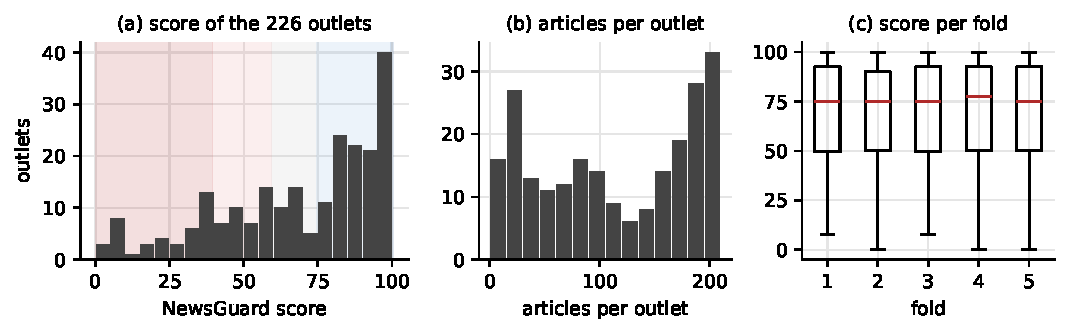
\includegraphics[width=\linewidth]{figures/dataset.pdf}
\caption{The 226 outlets: (a) NewsGuard score, shaded by NewsGuard level; (b) articles per outlet; (c) score in the
five folds of the outlet-disjoint split.}\label{fig:dataset}
\end{figure}

\subsection{Anonymization}\label{sec:anon}
A model could predict the score by recognizing the outlet (its name, its journalists, its links) rather than by
reading the text. Every title and text goes through three passes, each replacing spans with a placeholder and never
rewriting the text:
\begin{enumerate}
  \item links and e-mail addresses $\rightarrow$ \texttt{[URL]}, \texttt{[EMAIL]} (regular expressions);
  \item the outlet's own name, derived from its domain and written joined or spaced, with or without ``the''
        $\rightarrow$ \texttt{[OUTLET]} (a name that is also a common English word is replaced only when
        capitalized);
  \item GLiNER \citep{zaratiana2024gliner} (\texttt{gliner\_large-v2.1}, threshold 0.5), a zero-shot named-entity
        recognizer, with the labels \emph{news outlet} $\rightarrow$ \texttt{[OUTLET]} and \emph{journalist}
        $\rightarrow$ \texttt{[AUTHOR]}, applied to windows of 200 words.
\end{enumerate}
The third pass masks \emph{every} outlet and journalist, not only the publisher: citing another outlet (``according to
CNN'') can reveal the publisher's position in the media landscape, and the recognizer cannot tell the publisher's own
staff from other journalists. Passes 1--2 are needed because the recognizer alone leaves the outlet's own name in
about one article in four. After anonymization, \fillme\% of the articles still contain the name of their own outlet
\todo{fill from notebook 03; GLiNER: \fillme\ outlet and \fillme\ journalist spans in \fillme\% of the articles}.
Writing style, topics and political stance are not removed: they are the signal we study.

% =====================================================================================================================
\section{Method}\label{sec:method}

\begin{figure}[t]
\centering
\resizebox{\linewidth}{!}{%
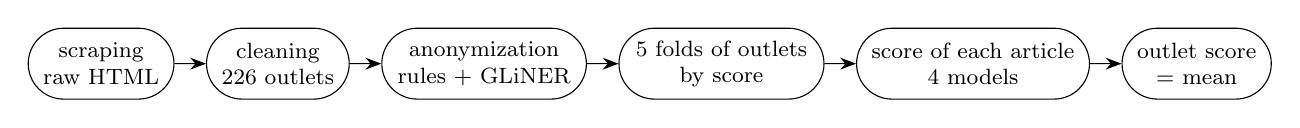
\begin{tikzpicture}[node distance=4mm, box/.style={draw, rounded rectangle, align=center, font=\footnotesize,
  minimum height=9mm, inner sep=3pt}, >={Stealth[length=2mm]}]
\node[box] (s) {scraping\\raw HTML};
\node[box, right=of s] (c) {cleaning\\226 outlets};
\node[box, right=of c] (a) {anonymization\\rules + GLiNER};
\node[box, right=of a] (f) {5 folds of outlets\\by score};
\node[box, right=of f] (m) {score of each article\\4 models};
\node[box, right=of m] (o) {outlet score\\= mean};
\foreach \x/\y in {s/c, c/a, a/f, f/m, m/o} \draw[->] (\x) -- (\y);
\end{tikzpicture}}
\caption{The pipeline.}\label{fig:pipeline}
\end{figure}

\subsection{Task and split}
Each outlet has one NewsGuard score $y \in [0, 100]$, assigned to all its articles. A model predicts a score for every
article; the score of an outlet is the mean of the predictions for its articles. Outlets are split into five folds:
outlets are sorted by score and, in consecutive blocks of five, each one goes to a different fold at random, so that
every fold has the same score distribution (Figure~\ref{fig:dataset}c). An outlet, with all its articles, is always
in a single fold, and outlets of the same owner were already reduced to one. Every model is trained on four folds and
tested on the fifth; hyper-parameters are chosen with three inner folds of the training outlets, built the same way.

\subsection{Models}
\begin{description}
  \item[TF-IDF.] Word uni- and bi-grams (at most 100,000, minimum document frequency 5, sublinear term frequency),
        fitted on the training articles, and a ridge regression; the penalty is chosen on the inner folds by the
        Spearman correlation per outlet.
  \item[Qwen3-Embedding-8B, frozen.] The embedding model \citep{zhang2025qwen3} reads every article in full with an
        instruction (\emph{``represent this news article to judge the reliability and journalistic standards of the
        outlet that published it''}); the vector of the last token, normalized, feeds a ridge regression on
        standardized features.
  \item[Mistral-Small-24B, frozen.] The base language model \citep{mistralsmall} (4-bit quantization) reads every
        article; the mean of the hidden states of layer 27 (of 40) over the article's tokens feeds a ridge
        regression, as above. \todo{say why layer 27.}
  \item[ModernBERT, fine-tuned.] ModernBERT-base \citep{warner2024modernbert} is trained end to end to regress the
        score (squared error on score/100; 5 epochs, learning rate $3\cdot10^{-5}$, effective batch 32).
\end{description}
No article is truncated: the longest one has about 3,000 tokens, below the 4,096 tokens read by every model.
\todo{all seeds fixed; hardware: one V100 32 GB.}

\subsection{Evaluation}
All measures are computed per outlet, on the 226 outlets of the five test folds: Spearman's $\rho$ and Kendall's
$\tau_b$ between predicted and true scores (the ranking of outlets), the mean absolute error (MAE, in points) and the
share of outlets predicted within 20 points of their score. The no-text baseline predicts, for every test outlet, the
mean score of the training outlets. Intervals are 95\% bootstrap intervals over outlets; differences between two
models are paired (same resampled outlets). To measure how many articles are needed, the score of each outlet is
also predicted from $k = 1, 2, 3, 5, 10, 20, 50$ random articles (20 draws per $k$, the same for every model).

% =====================================================================================================================
\section{Results}\label{sec:results}

\subsection{Main results}
\todo{fill from notebooks 08--09 (regressor rows only; predicted score, not stretched).}

\begin{table}[t]
\centering
\caption{Predicting the NewsGuard score of unseen outlets (226 outlets, all articles). 95\% bootstrap intervals in
brackets; $^\ast$: significantly better than TF-IDF (paired bootstrap).}\label{tab:main}
\begin{tabular}{lcccc}
\toprule
model & Spearman $\rho$ & Kendall $\tau_b$ & MAE (points) & within 20 (\%) \\
\midrule
no text (training mean) & -- & -- & \fillme & \fillme \\
TF-IDF + ridge & \fillme & \fillme & \fillme & \fillme \\
Qwen3-Embedding-8B (frozen) + ridge & \fillme & \fillme & \fillme & \fillme \\
Mistral-Small-24B (frozen) + ridge & \fillme & \fillme & \fillme & \fillme \\
ModernBERT (fine-tuned) & \fillme & \fillme & \fillme & \fillme \\
\bottomrule
\end{tabular}
\end{table}

\subsection{How many articles are needed}
\IfFileExists{figures/curves.pdf}{%
\begin{figure}[t]
\centering
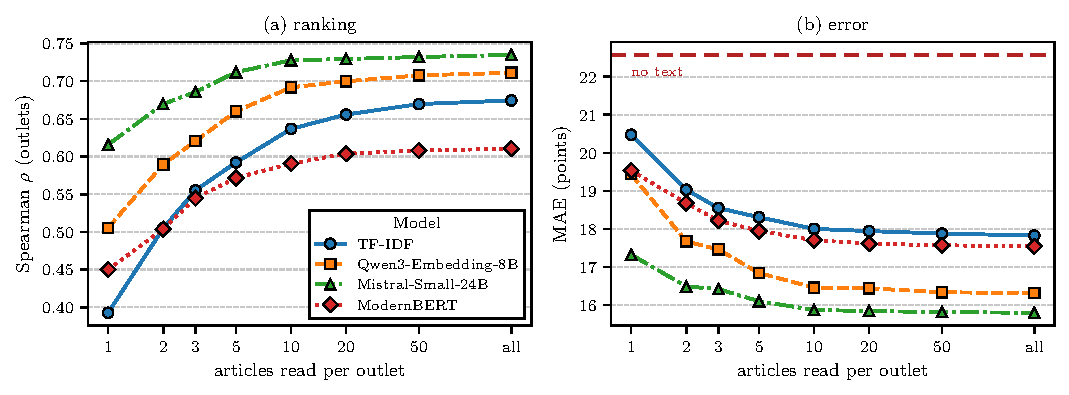
\includegraphics[width=\linewidth]{figures/curves.pdf}
\caption{Spearman correlation and MAE per outlet as a function of the number of articles read per outlet (mean of 20
random draws).}\label{fig:curves}
\end{figure}}{%
\begin{figure}[t]
\centering
\placeholder{0.9\linewidth}{4.5cm}
\caption{Spearman correlation and MAE per outlet as a function of the number of articles read per outlet.}
\label{fig:curves}
\end{figure}}
\todo{comment Figure~\ref{fig:curves}: with how many articles each model beats TF-IDF.}

\subsection{Robustness to the anonymization}
\todo{fill from notebook 12: the same models with a simpler anonymization (rules only: outlet name, signature, links,
own authors) against the anonymization of Section~\ref{sec:anon}; if the results barely change, the models do not rely
on explicit identifiers.}

\begin{table}[t]
\centering
\caption{Spearman $\rho$ and MAE per outlet with two anonymizations (all articles).}\label{tab:anon}
\begin{tabular}{lcccc}
\toprule
& \multicolumn{2}{c}{rules only} & \multicolumn{2}{c}{rules + GLiNER} \\
\cmidrule(lr){2-3}\cmidrule(lr){4-5}
model & $\rho$ & MAE & $\rho$ & MAE \\
\midrule
TF-IDF & \fillme & \fillme & \fillme & \fillme \\
Qwen3-Embedding-8B & \fillme & \fillme & \fillme & \fillme \\
Mistral-Small-24B & \fillme & \fillme & \fillme & \fillme \\
ModernBERT & \fillme & \fillme & \fillme & \fillme \\
\bottomrule
\end{tabular}
\end{table}

\subsection{Where the models err}
\todo{optional: errors by NewsGuard level (scores compressed towards the centre: the least reliable outlets are
overestimated, the most reliable underestimated).}

% =====================================================================================================================
\section{Discussion}\label{sec:discussion}
\todo{What the results mean: frozen large language models vs TF-IDF vs fine-tuned encoder; the ceiling of text-only
prediction (criteria such as ownership disclosure or corrections are not visible in the articles); use as a
screening tool for raters (rank outlets to review first).}

\paragraph{Limitations.}
\todo{one rater (NewsGuard) and one time point; political English-language outlets only; 226 outlets (small number of
independent units); the anonymization cannot remove style, which may itself identify an outlet; scores are
compressed towards the centre.}

\paragraph{Ethics and data availability.}
\todo{NewsGuard labels are licensed and not redistributable; we release code, article ids and URLs, and models; the method should support, not replace, human raters.}

% =====================================================================================================================
\section{Conclusion}\label{sec:conclusion}
\todo{two or three sentences.}

\bibliographystyle{plainnat}
\bibliography{references}

\end{document}
